\documentclass[a4paper,twocolumn,10pt,fleqn]{book}
\usepackage[american,ngerman]{babel}     %american / ngerman
\usepackage[T1]{fontenc}       %Silbentrennung
\usepackage[utf8]{inputenc}
%\usepackage[latin1]{inputenc}  %Direkteingabe von Umlauten
\usepackage{tabularx}
\usepackage{multirow}
\usepackage{colortbl}
\usepackage{longtable}
\usepackage{graphicx}
\usepackage{times}       %Erzwingt Typ 1 Schrift (skalierbar, gutes pdf-Output)
\usepackage[round,colon,authoryear]{natbib}      %Fuer Zitate mit \citep, \citet
\usepackage[fleqn]{amsmath}  % für \align-environment (ausgerichtete Gleichungen)
\usepackage{wasysym}  % common symbols (math + text mode), e.g. \permil
\usepackage{fancyhdr} % Customized header/footer
\usepackage{titling}
\usepackage{fink}
\usepackage{listings}
\usepackage{xcolor}
\usepackage{framed}
\usepackage{amsmath}
\usepackage{placeins}
\usepackage{makeidx}
\usepackage{rotfloat}
\usepackage[hyphens,obeyspaces]{url}


%Unterdrueckung von Hurenkindern und Schusterjungen
\clubpenalty = 10000
\widowpenalty = 10000 \displaywidowpenalty = 10000

% Vertiacal spacing between multi-line equations (e.g. in align env.)
\setlength{\jot}{11pt}

\def\arraystretch{1.2}

%%%%%%%%%%%%%%%%%%%%%%%%%%%%%%%%%%%%%%%%%%%%%%%%%%%%%%%%%
%%%%%%%%%%%%%%%%%%%%%% DEFINITIONS %%%%%%%%%%%%%%%%%%%%%%
%%%%%%%%%%%%%%%%%%%%%%%%%%%%%%%%%%%%%%%%%%%%%%%%%%%%%%%%%

%%%%%%%%%%%%%%%%%%%%%%%%%%%%%%%%%%%%%%%%%
% Optionen f�r die PDF-Erstellung 
%
% Achtung: Der Postprocessor dvips muss
%   mit der Option -z ausgef�hrt werden.
%%%%%%%%%%%%%%%%%%%%%%%%%%%%%%%%%%%%%%%%%
\usepackage[ps2pdf]{hyperref}
\usepackage{breakurl}
\definecolor{darkblue}{rgb}{0.2,0.2,0.8}
\hypersetup{%
colorlinks=true,        % Einfaerbung von Verknuepfungen
linkcolor=darkblue,     %Farbe dokumentinterner Links
citecolor=darkblue,     %Farbe dokumentinterner Links
bookmarksopen=false,    % Anzeige aller Ebenen
bookmarksnumbered=true, % Anzeige der Abschnittsnummern
pdfstartpage={1},       % Startseite
breaklinks=true
}

\usepackage[textfont={small,sl},labelfont={small,bf,sl},indention=0cm,singlelinecheck=false]{caption}
\captionsetup[figure]{position=bottom}
\captionsetup[table]{position=top}

%% Here it is: the code that adjusts justification and spacing around caption.
%% http://www.texnik.de/floats/caption.phtml
%\makeatletter
%% This does spacing around caption.
%\setlength{\abovecaptionskip}{0.3cm}
%\setlength{\belowcaptionskip}{0.3cm}
%% This does justification (left) of caption.
%\long\def\@makecaption#1#2{%
%  \vskip\abovecaptionskip
%  \sbox\@tempboxa{#1: #2}%
%  \ifdim \wd\@tempboxa >\hsize
%    #1: #2\par
%  \else
%    \global \@minipagefalse
%    \hb@xt@\hsize{\box\@tempboxa\hfil}%
%  \fi
%  \vskip\belowcaptionskip}
%\makeatother

% These commands are redefined in each chapter
\newcommand{\tabdir}{UNDEFINED}
\newcommand{\figdir}{UNDEFINED}

\newcommand{\tabref}[1]{Table~\ref{#1}}
\newcommand{\tabsref}[1]{Tables~\ref{#1}}
\newcommand{\figref}[1]{Fig.~\ref{#1}}
\newcommand{\figsref}[1]{Figs.~\ref{#1}}
\newcommand{\eqnref}[1]{Eqn.~\ref{#1}}
\newcommand{\eqnsref}[1]{Eqns.~\ref{#1}}
\newcommand{\appref}[1]{Appendix~\ref{#1}}
\newcommand{\secref}[1]{Sec.~\ref{#1}}
\newcommand{\secsref}[1]{Sections~\ref{#1}}
\newcommand{\chapref}[1]{Chap.~\ref{#1}}
\newcommand{\chapsref}[1]{Chapters~\ref{#1}}

\newenvironment{enumeratePacked}{
\begin{enumerate}
  \setlength{\itemsep}{4pt}
  \setlength{\parskip}{0pt}
  \setlength{\parsep}{0pt}
}{\end{enumerate}}

\newenvironment{itemizePacked}{
\begin{itemize}
  \setlength{\itemsep}{4pt}
  \setlength{\parskip}{0pt}
  \setlength{\parsep}{0pt}
}{\end{itemize}}

\newenvironment{descriptionPacked}{
\begin{description}
  \setlength{\itemsep}{4pt}
  \setlength{\parskip}{0pt}
  \setlength{\parsep}{0pt}
}{\end{description}}

% A command to produce an emphasized header on a single line
\newcommand{\desclisthead}[1]{\par\medskip\noindent\textit{\textbf{#1}}\\*\noindent}

% Modifies the format of the label in description environments (boldface --> italic)
\renewcommand{\descriptionlabel}[1]%
         {\hspace{\labelsep}\textit{#1}}

% Description env. with tt-Font label
\newcommand\mydescriptionlabel[1]{\hspace{\labelsep}\texttt{#1}}
\newenvironment{columndef}{%
   \let\descriptionlabel\mydescriptionlabel
   \description
}{%
   \enddescription
}

% An environment for the chapter introduction
\newenvironment{chapterintro}{
\begin{minipage}{0.75\textwidth}\slshape
}{\upshape \end{minipage}\twocolumn}


%%%%%%%%%%%%%%%%%%%%%%%%%%%%%%%%%%%%%%%%%%%%%%%%%%%%%%%%%%%%%%%%%%%%%%%%%%%%%
% COLOR DEFINITIONS
%%%%%%%%%%%%%%%%%%%%%%%%%%%%%%%%%%%%%%%%%%%%%%%%%%%%%%%%%%%%%%%%%%%%%%%%%%%%%

\definecolor{black}{rgb}{0,0,0}
\definecolor{darkgrey}{rgb}{0.2,0.2,0.2}
\definecolor{darkblue}{rgb}{0,0,0.7}
\definecolor{listnumbercolor}{rgb}{0.5,0.5,0.5}
\definecolor{brown}{rgb}{0.5,0.2,0}
\definecolor{magenta}{rgb}{0.7,0,0.4}

\definecolor{lightyellow}{rgb}{1.,1.,0.75}
\definecolor{lightblue}{rgb}{0.95,0.95,1}

%%%%%%%%%%%%%%%%%%%%%%%%%%%%%%%%%%%%%%%%%%%%%%%%%%%%%%%%%%%%%%%%%%%%%%%%%%%%%
% LANGUAGE DEFINITIONS
%%%%%%%%%%%%%%%%%%%%%%%%%%%%%%%%%%%%%%%%%%%%%%%%%%%%%%%%%%%%%%%%%%%%%%%%%%%%%

\lstdefinelanguage{txt}[]{}{%
  morecomment=[l]{\#}
}

%\lstloadlanguages{R}
\lstdefinelanguage{Renhanced}[]{R}{%
  morekeywords={colMeans,colSums,data.frame,dyn.load,dyn.unload,%
    in,is.na,is.null,is.finite,%
    mapply,na.rm,read.table,rep,rowMeans,rowSums,%
    which.max,which.min,write.table},
  deletekeywords={by,case,dir,dt,col,data,file,model,offset,par,sample,t,time},
  otherkeywords={!, \{, \}}, % Makes operators not keywords
  alsoletter={_.\%},
  alsoother={:\$},
  emph=[1]{TRUE,FALSE,NULL,NA,INF},
  morecomment=[is]{\#\#BeginHide}{\#\#EndHide}
}

%%%%%%%%%%%%%%%%%%%%%%%%%%%%%%%%%%%%%%%%%%%%%%%%%%%%%%%%%%%%%%%%%%%%%%%%%%%%%
% GENERIC STYLE DEFINITIONS
%%%%%%%%%%%%%%%%%%%%%%%%%%%%%%%%%%%%%%%%%%%%%%%%%%%%%%%%%%%%%%%%%%%%%%%%%%%%%

\lstdefinestyle{source}{extendedchars=true,
  basicstyle=\color{black}\ttfamily\small,
  commentstyle=\color{darkgrey}\textsl,
  keywordstyle=\color{darkblue}\textbf,
  stringstyle=\color{brown},
  emphstyle=[1]\color{magenta},
  showstringspaces=false,
  framexleftmargin=0mm,
  frame=shadowbox,
  rulesepcolor=\color{darkgrey},
  backgroundcolor=\color{lightblue},
  rulecolor=\color{lightblue},
  fillcolor=\color{lightblue}
%  numbers=left,
%  numberstyle=\color{darkgrey}\ttfamily\tiny,
%  stepnumber=1,
%  numbersep=3mm
}

\lstdefinestyle{data}{extendedchars=true,
  basicstyle=\color{black}\ttfamily\small,
  commentstyle=\color{darkgrey}\textsl,
  keywordstyle=\color{darkblue}\textbf,
  stringstyle=\color{brown},
  emphstyle=[1]\color{magenta},
  showstringspaces=false,
  framexleftmargin=0mm,
  frame=shadowbox,
  rulesepcolor=\color{darkgrey},
  backgroundcolor=\color{lightyellow},
  rulecolor=\color{lightyellow},
  fillcolor=\color{lightyellow}
%  numbers=left,
%  numberstyle=\color{darkgrey}\ttfamily\tiny,
%  stepnumber=1,
%  numbersep=3mm
}

%%%%%%%%%%%%%%%%%%%%%%%%%%%%%%%%%%%%%%%%%%%%%%%%%%%%%%%%%%%%%%%%%%%%%%%%%%%%%
% ACTUALLY USED STYLES
%%%%%%%%%%%%%%%%%%%%%%%%%%%%%%%%%%%%%%%%%%%%%%%%%%%%%%%%%%%%%%%%%%%%%%%%%%%%%

\lstdefinestyle{R}{language=Renhanced,style=source}
\lstdefinestyle{r}{language=Renhanced,style=source}

\lstdefinestyle{C++}{language=C++,style=source}
\lstdefinestyle{c++}{language=C++,style=source}
\lstdefinestyle{cpp}{language=C++,style=source}

\lstdefinestyle{shell}{language=bash,style=source}

\lstdefinestyle{txt}{language=txt,style=data}
\lstdefinestyle{text}{language=txt,style=data}

\hyphenation{ben-thic}
\hyphenation{ben-thal}
\hyphenation{Be-wert-ungs-skala}
\hyphenation{cyano-bac-teria}
\hyphenation{eu-tro-phic}
\hyphenation{eu-tro-phic-ation}
\hyphenation{de-ni-tri-fica-tion}
\hyphenation{dia-tom}
\hyphenation{dia-toms}
\hyphenation{hydro-graph}
\hyphenation{hydro-graphs}
\hyphenation{hypo-rheic}
\hyphenation{hypo-rheal}
\hyphenation{inter-stitial}
\hyphenation{macro-phyte}
\hyphenation{macro-phytes}
\hyphenation{pelagic}
\hyphenation{pelagial}
\hyphenation{phyto-plankton}
\hyphenation{ripa-rian}
\hyphenation{zoo-plankton}


\newcommand{\software}[1]{\texttt{\textbf{#1}}}

\newcommand{\function}[1]{\texttt{#1}}


%%%%%%%%%%%%%%%%%%%%%%%%%%%%%%%%%%%%%%%%%%%%%%%%%%%%%%%%%%%%%%%%%%%%%%%%%%%%%%%%
% MISCELLANEOUS
%%%%%%%%%%%%%%%%%%%%%%%%%%%%%%%%%%%%%%%%%%%%%%%%%%%%%%%%%%%%%%%%%%%%%%%%%%%%%%%%

% Real abbreviations
\newcommand{\ie}{i.~e.}
\newcommand{\eg}{e.~g.}

\newcommand{\first}{\ensuremath{1^{\rm st}}}  %1st
\newcommand{\second}{\ensuremath{2^{\rm nd}}}  %2nd

% Sub- and superscripts ...
\newcommand{\h}[1]{\ensuremath{^{\rm #1}}}  %superscript
\renewcommand{\l}[1]{\ensuremath{_{\rm #1}}}  %subscript
\newcommand{\e}[1]{\ensuremath{\cdot 10^{\rm #1}}}  % produces "*10^{arg}

% Typical math symbols
\newcommand{\deltat}{\ensuremath{\Delta t}}
\newcommand{\deltax}{\ensuremath{\Delta x}}
\newcommand{\average}{\ensuremath{\rm \overline{x}}}

\newcommand{\halflife}{\ensuremath{\tau}}

\newcommand{\tinc}{\texttt{t\_inc}}
\newcommand{\tbeg}{\texttt{t\_beg}}
\newcommand{\tend}{\texttt{t\_end}}



% Locigal values
\newcommand{\true}{\textsc{true}}
\newcommand{\false}{\textsc{false}}



%%%%%%%%%%%%%%%%%%%%%%%%%%%%%%%%%%%%%%%%%%%%%%%%%%%%%%%%%%%%%%%%%%%%%%%%%%%%%%%%
% HYDRO-METEOROLOGICAL VARIABLES
%%%%%%%%%%%%%%%%%%%%%%%%%%%%%%%%%%%%%%%%%%%%%%%%%%%%%%%%%%%%%%%%%%%%%%%%%%%%%%%%

% Basic meteorological variables
\newcommand{\precipIntensity}{\ensuremath{PI}}
\newcommand{\windspeed}{\ensuremath{WS}}
\newcommand{\airtemp}{\ensuremath{TA}}
\newcommand{\airPressure}{\ensuremath{PA}}
\newcommand{\relHumidity}{\ensuremath{RH}}
\newcommand{\solarRadiation}{\ensuremath{SR}}

% Variables related to moisture / humidity
\newcommand{\specHumidity}{\ensuremath{q}}
\newcommand{\specHumiditySurface}{\ensuremath{q_s}}
\newcommand{\vaporPressure}{\ensuremath{e}}
\newcommand{\vaporPressureSurface}{\ensuremath{e_s}}
\newcommand{\satVaporPressure}{\ensuremath{E}}
\newcommand{\satVaporPressureIce}{\ensuremath{E_i}}
\newcommand{\satVaporPressureWater}{\ensuremath{E_w}}

% Other meteorological variables
\newcommand{\cloudFraction}{\ensuremath{FC}}
\newcommand{\dewpointTemperature}{\ensuremath{T_{dew}}}

% Common (unspecific) hydrometeorological variables
\newcommand{\temperature}{\ensuremath{T}}

% Snow variables
\newcommand{\snowWaterEquivalent}{\ensuremath{SWE}}
\newcommand{\snowHeight}{\ensuremath{SH}}
\newcommand{\snowEnergyContent}{\ensuremath{SEC}}
\newcommand{\snowTemperature}{\ensuremath{T_s}}
\newcommand{\snowSurfaceTemperature}{\ensuremath{T_{ss}}}
\newcommand{\snowFractionLiquid}{\ensuremath{SLF}}
\newcommand{\snowRelSaturation}{\ensuremath{RSS}}

%%%%%%%%%%%%%%%%%%%%%%%%%%%%%%%%%%%%%%%%%%%%%%%%%%%%%%%%%%%%%%%%%%%%%%%%%%%%%%%%
% HYDRO-METEOROLOGICAL PROCESS RATES AND RELATED CONVERSION FACTORS
%%%%%%%%%%%%%%%%%%%%%%%%%%%%%%%%%%%%%%%%%%%%%%%%%%%%%%%%%%%%%%%%%%%%%%%%%%%%%%%%

% Energy fluxes
\newcommand{\netRadiationShort}{\ensuremath{R_{netS}}}
\newcommand{\netRadiationLong}{\ensuremath{R_{netL}}}
\newcommand{\heatfluxSens}{\ensuremath{R_{sens}}}
\newcommand{\heatfluxSoil}{\ensuremath{R_{soil}}}

\newcommand{\radLongwaveOut}{\ensuremath{R_{outL}}}
\newcommand{\radLongwaveIn}{\ensuremath{R_{inL}}}
\newcommand{\radLongwaveInClearsky}{\ensuremath{R_{inL,cs}}}
\newcommand{\radLongwaveInClouds}{\ensuremath{R_{inL,cl}}}

\newcommand{\radShortwaveIn}{\ensuremath{R_{inS}}}

% Mass fluxes
\newcommand{\massfluxPrec}{\ensuremath{M_{prec}}}
\newcommand{\massfluxSubl}{\ensuremath{M_{subl}}}
\newcommand{\massfluxFlow}{\ensuremath{M_{flow}}}

% Others
\newcommand{\albedoChangeRate}{\ensuremath{G_{alb}}}

%%%%%%%%%%%%%%%%%%%%%%%%%%%%%%%%%%%%%%%%%%%%%%%%%%%%%%%%%%%%%%%%%%%%%%%%%%%%%%%%
% PHYSICAL CONSTANTS AND CONCEPTUAL PARAMETERS USED IN HYDRO-METEOROLOGY
%%%%%%%%%%%%%%%%%%%%%%%%%%%%%%%%%%%%%%%%%%%%%%%%%%%%%%%%%%%%%%%%%%%%%%%%%%%%%%%%

% Densities
\newcommand{\densityWater}{\ensuremath{\rho_{w}}}
\newcommand{\densityIce}{\ensuremath{\rho_{i}}}
\newcommand{\densityAir}{\ensuremath{\rho_{a}}}
\newcommand{\densitySnow}{\ensuremath{\rho_{snow}}}
\newcommand{\densitySnowDry}{\ensuremath{\rho_{snow,dry}}}
\newcommand{\densitySoil}{\ensuremath{\rho_s}}

% Specific heat capacities
\newcommand{\specHeatWater}{\ensuremath{C_{wat}}}
\newcommand{\specHeatIce}{\ensuremath{C_{ice}}}
\newcommand{\specHeatAir}{\ensuremath{C_{air}}}
\newcommand{\specHeatSoil}{\ensuremath{C_s}}

% Latent heats
\newcommand{\evapHeatWater}{\ensuremath{E_{wat}}}
\newcommand{\evapHeatWaterZero}{\ensuremath{E_{wat,0}}}
\newcommand{\fusionHeatIce}{\ensuremath{H_{ice}}}
\newcommand{\sublimHeatIce}{\ensuremath{E_{ice}}}

% Radiation
\newcommand{\snowAlbedo}{\ensuremath{AS}}
\newcommand{\snowAlbedoMin}{\ensuremath{AS_{min}}}
\newcommand{\snowAlbedoMax}{\ensuremath{AS_{max}}}
\newcommand{\snowAlbedoRng}{\ensuremath{AS_{rng}}}

\newcommand{\stefanBoltzmann}{\ensuremath{\sigma}}
\newcommand{\emissivity}{\ensuremath{\varepsilon}}


% Stoichiometry factors and functions used in the snow model
\newcommand{\stoifacPrecMassToEnergy}{\ensuremath{f_{prec}}}
\newcommand{\stoifacSublMassToEnergy}{\ensuremath{f_{subl}}}
\newcommand{\stoifacFlowMassToEnergy}{\ensuremath{f_{flow}}}

% Various parameters of the snow model
\newcommand{\turbTransCoeff}{\ensuremath{D}}
\newcommand{\airtempRainSnow}{\ensuremath{T_{crit}}}
\newcommand{\soilInteractionDepth}{\ensuremath{D_s}}
\newcommand{\snowRelCapRetent}{\ensuremath{SCR}}
\newcommand{\snowSatHydrCond}{\ensuremath{k_{sat,snow}}}
\newcommand{\snowAlbedoDecrConst}{\ensuremath{k_{AS}}}
\newcommand{\leafAreaIndexFullShadow}{\ensuremath{LAI_{r0}}}

% Evapotranspiration
\newcommand{\etPot}{\ensuremath{et_{pot}}}
\newcommand{\etReal}{\ensuremath{et_{real}}}
\newcommand{\leafAreaIndex}{\ensuremath{LAI}}


%%%%%%%%%%%%%%%%%%%%%%%%%%%%%%%%%%%%%%%%%%%%%%%%%%%%%%%%%%%%%%%%%%%%%%%%%%%%%%%%
% CONSTANTS AND VARIABLES RELATED TO RUNOFF GENERATION AND -CONCENTRATION
%%%%%%%%%%%%%%%%%%%%%%%%%%%%%%%%%%%%%%%%%%%%%%%%%%%%%%%%%%%%%%%%%%%%%%%%%%%%%%%%

\newcommand{\soilWaterContent}{\ensuremath{\theta}}
\newcommand{\soilWaterContentMax}{\ensuremath{\theta_{max}}}

\newcommand{\relSat}{\ensuremath{S}}
\newcommand{\relSatInter}{\ensuremath{S_{int}}}
\newcommand{\relSatBase}{\ensuremath{S_{base}}}


\newcommand{\heightRunoffDirect}{\ensuremath{h_{d}}}

\newcommand{\rateRunoffSurf}{\ensuremath{r_{surf}}}
\newcommand{\rateRunoffPref}{\ensuremath{r_{pref}}}
\newcommand{\rateRunoffInter}{\ensuremath{r_{int}}}
\newcommand{\rateRunoffBase}{\ensuremath{r_{base}}}
\newcommand{\rateEvapotransp}{\ensuremath{r_{evap}}}
\newcommand{\rateSnowMelt}{\ensuremath{r_{melt}}}

\newcommand{\soilDepth}{\ensuremath{D}}
\newcommand{\satFrac}{\ensuremath{f_{sat}}}
\newcommand{\expSatFrac}{\ensuremath{{\beta}}}

\newcommand{\thresholdSurf}{\ensuremath{{thr_{surf}}}}

\newcommand{\rateWaterSupply}{\ensuremath{WS}}

\newcommand{\expInter}{\ensuremath{{E_{int}}}}
\newcommand{\expBase}{\ensuremath{{E_{base}}}}

\newcommand{\facInter}{\ensuremath{{b_{int}}}}
\newcommand{\facBase}{\ensuremath{{b_{base}}}}

\newcommand{\strSurf}{\ensuremath{{S_{surf}}}}
\newcommand{\strPref}{\ensuremath{{S_{pref}}}}
\newcommand{\strInter}{\ensuremath{{S_{inter}}}}
\newcommand{\strBase}{\ensuremath{{S_{base}}}}

\newcommand{\concTimeIndex}{\ensuremath{{CTI}}}

\newcommand{\satHydrCond}{\ensuremath{k_{f}}}



% IMPORTANT PHYSICAL UNITS

% Time
\newcommand{\persec}{s\ensuremath{^{-1}}}
\newcommand{\perday}{d\ensuremath{^{-1}}}

% Length
\newcommand{\perm}{m\ensuremath{^{-1}}}
\newcommand{\perdm}{dm\ensuremath{^{-1}}}
\newcommand{\percm}{cm\ensuremath{^{-1}}}
\newcommand{\permm}{mm\ensuremath{^{-1}}}

% Area
\newcommand{\sqkm}{km\ensuremath{^{2}}}
\newcommand{\sqm}{m\ensuremath{^{2}}}
\newcommand{\sqdm}{dm\ensuremath{^{2}}}
\newcommand{\sqcm}{cm\ensuremath{^{2}}}
\newcommand{\sqmm}{mm\ensuremath{^{2}}}

\newcommand{\persqm}{m\ensuremath{^{-2}}}
\newcommand{\persqdm}{dm\ensuremath{^{-2}}}
\newcommand{\persqcm}{cm\ensuremath{^{-2}}}
\newcommand{\persqmm}{mm\ensuremath{^{-2}}}

% Volume
\newcommand{\cbm}{m\ensuremath{^{3}}}
\newcommand{\cbdm}{dm\ensuremath{^{3}}}
\newcommand{\cbcm}{cm\ensuremath{^{3}}}
\newcommand{\cbmm}{mm\ensuremath{^{3}}}

\newcommand{\percbm}{m\ensuremath{^{-3}}}
\newcommand{\percbdm}{dm\ensuremath{^{-3}}}
\newcommand{\percbcm}{cm\ensuremath{^{-3}}}
\newcommand{\percbmm}{mm\ensuremath{^{-3}}}
\newcommand{\perlitre}{l\ensuremath{^{-1}}}

% Mass
\newcommand{\perkg}{kg\ensuremath{^{-1}}}
\newcommand{\perg}{g\ensuremath{^{-1}}}
\newcommand{\permg}{mg\ensuremath{^{-1}}}

% Flow
\newcommand{\cbms}{\cbm~\persec}

% Temperature
\newcommand{\celsius}{\ensuremath{^\circ}C}

\definecolor{shadecolor}{rgb}{0.9,0.9,0.9}


\addtolength{\evensidemargin}{-1cm}
\addtolength{\oddsidemargin}{+1cm}

\setcounter{tocdepth}{2}     % Numbers up to 0.0.0 in TOC     (chapter= 0, section= 1, subsection= 2 ...)
\setcounter{secnumdepth}{3}  % Numbers up to 0.0.0.0 in text  (chapter= 0, section= 1, subsection= 2 ...)

\arrayrulecolor{black}

\makeindex

\begin{document}

%%%%%%%%%%%%%%%%%%%%%%%%%%%%%%%%%%%%%%%%%%%%%%%%%%%%%%%%%
%%%%%%%%%%%%%%%%%%%%%% TITLE PAGES %%%%%%%%%%%%%%%%%%%%%%
%%%%%%%%%%%%%%%%%%%%%%%%%%%%%%%%%%%%%%%%%%%%%%%%%%%%%%%%%

\selectlanguage{american}
\pagestyle{empty}
\onecolumn

\begin{center}
  \vspace*{5cm}
  \LARGE
  \textbf{Eco-Hydrological Simulation Environment \\ (\software{echse})} \\
  \vspace*{1.2cm}
  Installation and Administration Guide \\
  \vspace*{2.0cm}
  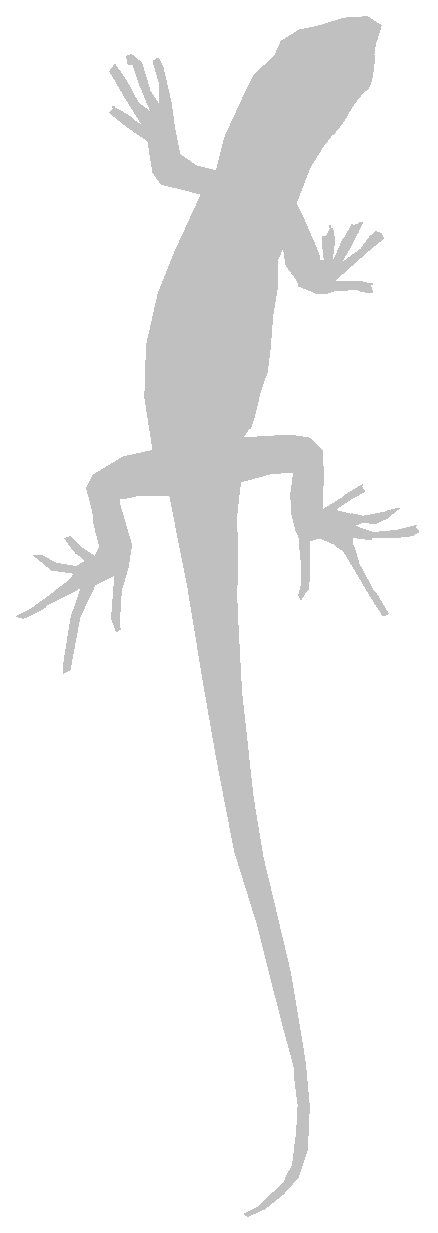
\includegraphics[width=0.1\textwidth,angle=270]{../../_common/fig/logo.eps}
\end{center}

\cleardoublepage

\vspace*{12cm}
\begin{tabular}{ll}
Author      & David Kneis \\
Affiliation & Institute of Earth and Environmental Sciences \\
            & Hydrology \& Climatology Section, \\
            & University of Potsdam, Germany \\
Contact     & david.kneis [at] uni-potsdam.de \\
            & \\
Project     & PROGRESS \\
Sub-project & D2.2 \\
Funding     & German Ministry of Education and Research (BMBF) \\
            & \\
Last update & \today{} \\
\end{tabular}

\vspace*{2.0cm}
\noindent Please help to improve this document by sending suggestions, corrections, wishes, and other useful feedback to the author (see above).

\cleardoublepage

%%%%%%%%%%%%%%%%%%%%%%%%%%%%%%%%%%%%%%%%%%%%%%%%%%%%%%%%%%
%%%%%%%%%%%%%%%%%%%%%% Page style   %%%%%%%%%%%%%%%%%%%%%%
%%%%%%%%%%%%%%%%%%%%%%%%%%%%%%%%%%%%%%%%%%%%%%%%%%%%%%%%%%

%%% Begin Fancy Header Settings
\pagestyle{fancy}                       % Sets fancy header and footer
\fancyfoot{}                            % Delete current footer settings
\renewcommand{\chaptermark}[1]{         % Lower Case Chapter marker style
  \markboth{\chaptername\ \thechapter\ \hspace{0.5cm} #1}{}}
\renewcommand{\sectionmark}[1]{         % Lower case Section marker style
  \markright{\thesection\ \hspace{0.5cm} #1}}
\fancyhead[LE,RO]{\bfseries\thepage}    % Page number (boldface) in left on even pages and right on odd pages
\fancyhead[RE]{\bfseries\leftmark}      % Chapter in the right on even pages
\fancyhead[LO]{\bfseries\rightmark}     % Section in the left on odd pages
\renewcommand{\headrulewidth}{0.3pt}    % Width of head rule %%% Clear Header
%% End Fancy Header Settings

%%%%%%%%%%%%%%%%%%%%%%%%%%%%%%%%%%%%%%%%%%%%%%%%%%%%%%%%%%
%%%%%%%%%%%%%%%%%%%%%% TOC          %%%%%%%%%%%%%%%%%%%%%%
%%%%%%%%%%%%%%%%%%%%%%%%%%%%%%%%%%%%%%%%%%%%%%%%%%%%%%%%%%

%% Begin TOC Settings
\pdfbookmark[1]{\contentsname}{toc}
\fancyhead[LE,RO]{\bfseries\thepage}
\fancyhead[RE]{\bfseries Contents}
\fancyhead[LO]{\bfseries Contents}
\tableofcontents
%% End TOC Settings

%%%%%%%%%%%%%%%%%%%%%%%%%%%%%%%%%%%%%%%%%%%%%%%%%%%%%%
%%%%%%%%%%%%%%%%%%%%%% ABSTACTS %%%%%%%%%%%%%%%%%%%%%%
%%%%%%%%%%%%%%%%%%%%%%%%%%%%%%%%%%%%%%%%%%%%%%%%%%%%%%

\onecolumn

% English summary
%\cleardoublepage
%\fancyhead[LE,RO]{\bfseries\thepage}
%\fancyhead[RE]{ }
%\fancyhead[LO]{ }
%\selectlanguage{american}
%\section*{Abstract}
\addcontentsline{toc}{chapter}{Abstract}

English abstract.



% German dummary
%\cleardoublepage
%\fancyhead[LE,RO]{\bfseries\thepage}
%\fancyhead[RE]{ }
%\fancyhead[LO]{ }
%\selectlanguage{ngerman}
%\section*{Kurzfassung}
\addcontentsline{toc}{chapter}{German abstract}

Deutsches Abstract.


%\selectlanguage{american}
%\cleardoublepage

%%%%%%%%%%%%%%%%%%%%%%%%%%%%%%%%%%%%%%%%%%%%%%%%%%%%%%%%%%
%%%%%%%%%%%%%%%%%%%%%% THE CHAPTERS %%%%%%%%%%%%%%%%%%%%%%
%%%%%%%%%%%%%%%%%%%%%%%%%%%%%%%%%%%%%%%%%%%%%%%%%%%%%%%%%%

\onecolumn

% Reestablish header
\fancyhead[LE,RO]{\bfseries\thepage}    % Page number (boldface) in left on even pages and right on odd pages
\fancyhead[RE]{\bfseries\leftmark}      % Chapter in the right on even pages
\fancyhead[LO]{\bfseries\rightmark}     % Section in the left on odd pages

%%%%% Chapter sources

\chapter{Required external software} \label{chap:extSoft}
\renewcommand{\tabdir}{chapters/extSoft/extSoft/tab}
\renewcommand{\figdir}{chapters/extSoft/extSoft/fig}

%%%%%%%%%%%%%%%%%%%%%%%%%%%%%%%%%%%%%%%%%%%%%%%%%%%%%%%%%%%%%%%%%%%%%%%%%%%%%%%%
\section{Before installing software} \label{sec:extSoft:generalNotes}
Be aware of the fact that the installation of any software, in particular if downloaded from the internet, is a potentially dangerous. If you install the suggested software, you do this at your own risk! To minimize the risk, it is recommended that you
\begin{itemize}
  \item download the software from their official websites.
  \item scan downloaded files for viruses before execution.
  \item make regular backups of all important files to be prepared even for the worst case.
\end{itemize}

Note that you probably need administrator privileges to successfully install any of the software tools mentioned in the subsequent sections.

%%%%%%%%%%%%%%%%%%%%%%%%%%%%%%%%%%%%%%%%%%%%%%%%%%%%%%%%%%%%%%%%%%%%%%%%%%%%%%%%
\section{Statistical computing software 'R'} \label{sec:extSoft:R}

\subsection{What is it good for?} \label{sec:extSoft:R:why}
Most of the \software{echse}-related pre- and post-processing tools are implemented in the R language. The \software{echse}'s code generator is currently implementend as an R-package too.

\subsection{Basic installation} \label{sec:extSoft:R:basic}
R is a widely used software for statistical computing and graphics creation \citep{R}. It is freely available for most platforms, including Linux and Windows. The official address of the project is \url{http://www.r-project.org}.

To find out whether R is installed on your system, type \verb!R --version! at the command line. If R is available, a version info similar to the one shown below should appear.
\begin{lstlisting}[style=shell]
dkneis@teufelsturm:/$ R --version
R version 2.10.1 (2009-12-14)
Copyright (C) 2009 The R Foundation [...]
ISBN 3-900051-07-0
[...]
dkneis@teufelsturm:/$
\end{lstlisting}

If this is not the case, you need to install R. Linux users need to use the package manager or an appropriate apt-command. Users of Windows need to go through the following steps:

\begin{enumerate}
  \item Visit \url{http://www.r-project.org}
  \item Save the installer for the latest version. The file name should be like \verb!R-0.00.0-win.exe! (\verb!0.00.0! = version).
  \item Execute this file and follow the instructions.
  \item Update your \verb!PATH! environment variable to include the directory where the R binaries reside. If you installed R in folder \verb!c:\program files!, for example, this will typically be \verb!c:\program files\R\R-0.00.0\bin!. See Appendix \ref{chap:appendix:envVars} for information on how to set or modify environment variables.
  \item Open a \textbf{new} terminal and check for a proper installation by querying the R version (see instructions above).
\end{enumerate}

\subsection{Installation of add-on packages} \label{sec:extSoft:R:packages}

For some applications it may be necessary to install additional R-packages. These packages are not included in the basic R distribution and must be obtained separately.

\begin{description}
  \item[Officially published R packages] can be found on the CRAN website (CRAN: Comprehensive R Archive Network; see link at \url{http://www.r-project.org}). Typically, versions for several platforms and additional documentation material in PDF format is provided.
  \item[Other packages] which are non officially published on CRAN are most often distributed as so-called tarballs. These are compressed archive files with the file extension \verb!.tar.gz!.
\end{description}

On some systems (namely Windows), a menue is available at the top of the R console window that allows for convenient package installation, including download from CRAN. The system-independend way of package installation, however, uses the command line. Assuming that the package is available as a tarball, the following shell command should work on all platforms. In the example, 'pname' is the package name and 'x.y' is a version number.

\begin{lstlisting}[style=shell]
R CMD INSTALL pname_x.y.tar.gz
\end{lstlisting}

To check whether an add-on package is properly installed use the R commands \verb!library()! or \verb!require()!.

For more help on package installation either type \verb!?INSTALL! at the R prompt or use the shell command \verb!R CMD INSTALL --help! from a normal terminal. Experience shows that package installation on Windows systems is sometimes difficult. If the installation fails due to permission issues, one could try to open a terminal with administrator privileges and then run the \verb!R CMD INSTALL! command shown above.

Sometimes more difficulties arise if native source code (Fortran, C, C++) needs to be compiled during package installation. In such cases, the instructions given at \url{http://cran.r-project.org/doc/manuals/R-admin.html#The-Windows-toolset} may help. It seems that a common source of trouble is the existence of multiple parallel installations of a 'make' program or compilers (gfortran, gcc). In those cases, it may be necessary to modify the \verb!PATH! environment variable (put the R-related directories first).

%%%%%%%%%%%%%%%%%%%%%%%%%%%%%%%%%%%%%%%%%%%%%%%%%%%%%%%%%%%%%%%%%%%%%%%%%%%%%%%%

\section{The GNU C++ compiler 'g++'} \label{sec:extSoft:gpp}

\subsection{What is it good for?} \label{sec:extSoft:gpp:why}
g++ is the C++ compiler from the GNU compiler collection (gcc). It is a widely used, free software and runs on several platforms including Linux and Windows. It is used to compile the \software{echse}'s C++ source code. It may also be used to compile those pre- and/or post-processor tools which are implemented in C++.

\subsection{Installation} \label{sec:extSoft:gpp:basic}

To find out whether g++ is installed on your system, type \verb!g++ --ver! at the command line. If the compiler is available, a version info similar to the one shown below should appear.

\begin{lstlisting}[style=shell]
dkneis@teufelsturm:/$ g++ --ver
Using built-in specs.
Target: i486-linux-gnu
Configured with: ../src/configure -v     [...]
Thread model: posix
gcc version 4.4.3 (Ubuntu 4.4.3-4ubuntu5)
dkneis@teufelsturm:/$
\end{lstlisting}

If this is not the case, you need to install the g++ compiler. Linux users need to use the package manager or an appropriate apt-command. Users of Windows need to install MinGW and MSYS by going through the following steps:

\begin{enumerate}
  \item Remove an older MinGW version if present. This is normally achieved by deleting the entire MinGW folder. You should make sure, however, that no other applications depend on that old version.
  \item Visit \url{http://www.mingw.org}
  \item From the download area, save the latest version of the installer. The file name should be like \verb!mingw-get-inst-YYYYMMDD.exe! (\verb!YYYYMMDD! = a date).
  \item Execute this file. In the dialogue, select at least the following components for installation:
    \begin{itemize}
      \item MinGW compiler suite -- C++ compiler. This will install g++.
      \item MinGW developer toolkit including the MSYS basic system.
    \end{itemize}
  It is not a bad idea to also select the Fortran gfortran from the MinGW compiler suite for installation.
  \item The user-selected path of the installation directory should not contain blanks (recommended: \verb!c:/mingw!).
  \item Note that the installer first downloads many files. Thus, you need an active internet connection.
  \item Update your \verb!PATH! environment variable to include the two directories
    \begin{itemize}
      \item \verb!c:\mingw\bin! (contains MinGW binaries) and
      \item \verb!c:\mingw\msys\<x.y>\bin! (contains MSYS binaries)
    \end{itemize}
   where \verb!c:\mingw! is the assumed (and recommended) installation directory and \verb!<x.y>! is a version number. See Appendix \ref{chap:appendix:envVars} for information on how to set or modify environment variables.
  \item Open a \textbf{new} terminal and check for a proper installation by querying the version of g++ (see instructions above).
\end{enumerate}

%%%%%%%%%%%%%%%%%%%%%%%%%%%%%%%%%%%%%%%%%%%%%%%%%%%%%%%%%%%%%%%%%%%%%%%%%%%%%%%%

\section{The GNU Fortran compiler 'gfortran'} \label{sec:extSoft:gfortran}

\subsection{What is it good for?} \label{sec:extSoft:gfortran:why}
gfortran is the Fortran compiler of the GNU compiler collection (gcc). It supports the Fortran 95 standard (at least), it is freely available and widely used. The gfortran compiler is required to compile Fortran code used by \software{echse}-related pre- and/or post-processing tools, namely some R packages.

\subsection{Installation} \label{sec:extSoft:gfortran:basic}

To find out whether gfortran is installed on your system, type \verb!gfortran --version! at the command line. If the compiler is available, a version info similar to the one shown below should appear.
\begin{lstlisting}[style=shell]
dkneis@teufelsturm:/$ gfortran --version
GNU Fortran (Ubuntu 4.4.3-4ubuntu5) 4.4.3
Copyright (C) 2010 Free Software F[...]
[...]
dkneis@teufelsturm:/$
\end{lstlisting}

If this is not the case, you need to install gfortran. Linux users need to use the package manager or an appropriate apt-command. Users of Windows please go through all the steps described in the enumeration at the end of \secref{sec:extSoft:gpp}. In the dialog where you need to select components for installation, simply chose the Fortran compiler instead of (or in addition to) the C++ compiler.

%%%%%%%%%%%%%%%%%%%%%%%%%%%%%%%%%%%%%%%%%%%%%%%%%%%%%%%%%%%%%%%%%%%%%%%%%%%%%%%%

\section{MSYS (Windows users only)} \label{sec:extSoft:msys}

MSYS provides basic Linux command line utilities for use on Windows systems. Using MSYS, it is possible to execute Linux bash shell scripts also on Windows systems. If you installed the C++ compiler g++ following the instructions in \secref{sec:extSoft:gpp}, you should already have MSYS on your system. If not, please follow the instructions in \secref{sec:extSoft:gpp} and optionally skip the installation of a compiler.

If MSYS is properly installed, commands like \verb!pwd! or \verb!ls! should work when typed at a Windows command prompt. These commands show the current directory and list its contents, respectively.

%%%%%%%%%%%%%%%%%%%%%%%%%%%%%%%%%%%%%%%%%%%%%%%%%%%%%%%%%%%%%%%%%%%%%%%%%%%%%%%%

\section{A convenient text editor} \label{sec:extSoft:editor}

On Linux systems, appropriate text editors are installed by default. On Windows, the default editor is hardly usable for serious text editing. NOTEPAD++ appears to be a good and free alternative.


\chapter{Installation of model engines} \label{chap:install}
\renewcommand{\tabdir}{chapters/install/install/tab}
\renewcommand{\figdir}{chapters/install/install/fig}

\section{Introduction} \label{sec:install:intro}

This chapter deals with the installation of \software{echse}-based model engines from \emph{existing} source code. The chapter does not cover the topic of model development or modification. The information is addressed to users of both Linux and Windows.

In this context, the term \emph{model engine} is used to denote the binary file which is executed when performing a simulation. The term is introduced to allow for a clear distinction between the \emph{model engine} (plain binary file) and the \emph{model} (binary file + input data). 

%%%%%%%%%%%%%%%%%%%%%%%%%%%%%%%%%%%%%%%%%%%%%%%%%%%%%%%%%%%%%%%%%%%%%%%%%%%%%%
%%%%%%%%%%%%%%%%%%%%%%%%%%%%%%%%%%%%%%%%%%%%%%%%%%%%%%%%%%%%%%%%%%%%%%%%%%%%%%

\section{Software to install} \label{sec:install:software}

%%%%%%%%%%%%%%%%%%%%%%%%%%%%%%%%%%%%%%%%%%%%%%%%%%%%%%%%%%%%%%%%%%%%%%%%%%%%%%

\subsection{Programs}

You need to install the following programs in order to build an \software{echse}-based model engine:

\begin{itemize}
  \item The 'R' software for statistical computing.
  \item The GNU C++ compiler 'g++'.
  \item Windows users: The bash-shell interpreter and commands provided by 'MSYS'.
\end{itemize}

Linux users probably want to use the package manager to install the software. Windows users should try the installers which can be downloaded from the respective websites. Please follow the installation instructions given in \chapref{chap:extSoft} as closely as possible. In particular, on Windows systems, it is important to add the binary directories of all the software to the \verb!PATH! variable in order to make the programs accessible from any shell.

%%%%%%%%%%%%%%%%%%%%%%%%%%%%%%%%%%%%%%%%%%%%%%%%%%%%%%%%%%%%%%%%%%%%%%%%%%%%%%

\subsection{R-packages}

You need to install the R-package \software{codegen} in order to run the \software{echse}'s code generator. You should find the latest version of this package in the sub-folder \verb!R/packages! of the \software{echse}-tools main directory (see \secref{sec:install:folders}). The package is distributed as a tarball archive \verb!codegen_x.y.tar.gz! where \verb!x.y! is the current version number. See \secref{sec:extSoft:R:packages} for details on how to install R-packages.

%%%%%%%%%%%%%%%%%%%%%%%%%%%%%%%%%%%%%%%%%%%%%%%%%%%%%%%%%%%%%%%%%%%%%%%%%%%%%%
%%%%%%%%%%%%%%%%%%%%%%%%%%%%%%%%%%%%%%%%%%%%%%%%%%%%%%%%%%%%%%%%%%%%%%%%%%%%%%

\section{The \software{echse} standard folders} \label{sec:install:folders}

%%%%%%%%%%%%%%%%%%%%%%%%%%%%%%%%%%%%%%%%%%%%%%%%%%%%%%%%%%%%%%%%%%%%%%%%%%%%%%

\subsection{Overview} \label{sec:install:folders:overview}

At present, all \software{echse}-related files are split accross a small number of folders, also referred to as the \software{echse} \emph{standard folders}. These folders are briefly explained in \tabref{tab:install:folders}.

\begin{table}[h]
  \caption{The \software{echse} standard folders. \label{tab:install:folders}}  
  \begin{tabular}{p{0.2\textwidth}p{0.75\textwidth}} \hline\hline
     Folder & Contents \\ \hline
     \verb!echse_docs! & Documentations, mostly as \LaTeX{} projects. \\
     \verb!echse_generic! & Common C++ source code being used by all \software{echse}-based model engines. Also contains generic scripts for engine building. \\
     \verb!echse_engines! & C++ source code of the classes being used by one or more particular model engines. This includes both generated and manually written code. Also contains text files with class and model declarations. \\
     \verb!echse_tools! & \software{echse}-related tools for pre- and post-processing of data. \\
     \hline\hline
  \end{tabular}
\end{table}

It is assumed that you have obtained current versions of the \software{echse} standard folders listed in \tabref{tab:install:folders} either from repositories or by unpacking release archives. In order to install a model engine, you need at least the \verb!echse_generic! and \verb!echse_engines! folders whose contents is displayed in \figsref{fig:install:folders:generic} \& \ref{fig:install:folders:engines}, respectively. Note that only the most important branches are displayed in these figures.

\begin{figure}[h]
\begin{lstlisting}[style=text]
  echse_generic --+-- core
                  |
                  +-- cpplib
                  |
                  +-- scripts
\end{lstlisting}
  \caption{Main branches of the \software{echse} standard folder with generic files. \label{fig:install:folders:generic}}
\end{figure}

\begin{figure}[h]
\begin{lstlisting}[style=text]
  echse_engines --+-- bin
                  |
                  +-- classes
                  |
                  +-- def
                  |
                  +-- generated
                  |
                  +-- processes
\end{lstlisting}
\caption{Main branches of the \software{echse} standard folder with class files for particular model engines. \label{fig:install:folders:engines}}
\end{figure}

The functionality of many scripts and files contained in the folders \verb!echse_generic! and \verb!echse_engines! and its sub-folders depends on the integrity of the respective directory trees. Therefore, you should \emph{not} rename, move, or delete any of the sub-folders and files without considering the potential consequences. Note that all references to files and directories are \emph{relative}. Therefore, you can savely move each of the \software{echse} standard folders \emph{as a whole} as long as you keep your system informed on their locations (see \secref{sec:install:env:folders}).

%%%%%%%%%%%%%%%%%%%%%%%%%%%%%%%%%%%%%%%%%%%%%%%%%%%%%%%%%%%%%%%%%%%%%%%%%%%%%%

\subsection{Definition of model engines} \label{sec:install:folders:engines}

The following enumeration outlines the concept of model engines from a top-down point of view. It also gives a brief overview of the contents of the \software{echse} standard folder \verb!echse_engines!.

\begin{enumerate}
  \item Each model engine is composed of a particular set of classes. A rainfall-runoff model, for example, may comprise a sub-basin class, a reach class, and additional classes for special types of objects (reservoirs etc.). The set of classes being used in a particular model engines is listed in the text files in folder \verb!echse_engines/def!.
  \item Each of the classes is characterized by a particular set of data members (forcings, state variables, parameters, etc.). For each class, the declaration of data members can be found in the text files in folder \verb!echse_engines/classes/declaration!. See \citet{Echse-Main-Doc} for details.
  \item Class declaration and implementation are well separated. The declaration part of the classes' source code is created by the code generator (output in \verb!echse_engines/generated!). The implementation part consisting of manually written code to be found in \verb!echse_engines/classes/implementation! (C++ include files).
  \item The dynamics of state variables are due to the action of processes. In the \software{echse} concept, processes are represented by functions whose return value is typically a rate (mass or energy flux) or a derivative of a state variable with respect to time. Since a particular function may be used in multiple classes, the code is separated from the class implementation. It can be found in \verb!echse_engines/processes!
\end{enumerate}

%%%%%%%%%%%%%%%%%%%%%%%%%%%%%%%%%%%%%%%%%%%%%%%%%%%%%%%%%%%%%%%%%%%%%%%%%%%%%%
%%%%%%%%%%%%%%%%%%%%%%%%%%%%%%%%%%%%%%%%%%%%%%%%%%%%%%%%%%%%%%%%%%%%%%%%%%%%%%

\section{Environment variables to be set} \label{sec:install:env}

\subsection{Pointers to the \software{echse} standard folders} \label{sec:install:env:folders}
The \software{echse} is not a software in the classical sense and, therefore, it does not require the typical installation procedure. There is neither an installer nor is the \software{echse} distributed as an installable software package. In particular, on a Windows system, the \software{echse} does not integrate into the so-called 'registry'.

Any \software{echse}-related files are contained in the standard folders introduced in \secref{sec:install:folders}. All you need to do is to inform the system on the location of these folders. For that purpose, you must define the environment variables listed in \tabref{tab:install:env:folders}. Note that the variable names are UPPERCASE. See \appref{chap:appendix:envVars} and/or the help files of your operating system for detailed information on how to permanently set environment variables.

\begin{table}[h]
  \caption{Environment variables pointing to the \software{echse} standard folders. \label{tab:install:env:folders}}
  \begin{tabular}{p{0.2\textwidth}p{0.75\textwidth}} \hline\hline
    Variable name & Value \\ \hline
    \verb!ECHSE_GENERIC! & Full path of the \software{echse} standard folder \verb!echse_generic!. \\
    \verb!ECHSE_ENGINES! & Full path of the \software{echse} standard folder \verb!echse_engines!. \\
    \verb!ECHSE_TOOLS! & Full path of the \software{echse} standard folder \verb!echse_tools!. \\
    \hline\hline
  \end{tabular}
\end{table}

\begin{minipage}{0.15\textwidth}
  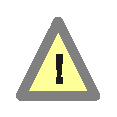
\includegraphics[width=0.6\textwidth]{../../_common/fig/symbols_warning.eps}   
\end{minipage}
\begin{minipage}{0.8\textwidth}
On Windows systems, you need to use the forward slash (\verb!/!) instead of the usual back-slash (\verb!\!) to separate directory names in the value of the environment variables listed in \tabref{tab:install:env:folders}. For example, if one of your \software{echse} standard folders is \verb!d:\modeling\echse_generic!, the proper value of \verb!ECHSE_GENERIC! would be \verb!d:/modeling/echse_generic!. Disregard of this will cause problems during the compilation of model engines.
\end{minipage} \\

\begin{minipage}{0.15\textwidth}
  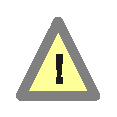
\includegraphics[width=0.6\textwidth]{../../_common/fig/symbols_warning.eps}   
\end{minipage}
\begin{minipage}{0.8\textwidth}
There must be no white space characters in the names of the \software{echse} standard folders. The existence of such characters (at any position) would break the functionality of some scripts. If you care for readability, use the \verb!_! character instead of white space, \ie{} use \verb!d:/my_files/echse_generic! instead of \verb!d:/my files/echse_generic!, for example. Disregard of this will cause problems during the compilation of model engines.
\end{minipage} \\

If you ever move one (or all) of the \software{echse} standard folder(s), the variables listed in \tabref{tab:install:env:folders} need to be updated to reflect the new location(s). If you follow the recommendations in \secref{sec:install:env:path}, no additional work is necessary.

\subsection{Adjusting the PATH variable} \label{sec:install:env:path}

Some sub-directories of the \software{echse} standard folders contain executable files (binaries and shell scripts). This is true in particular for the two folders \verb!echse_engines/bin! (\figref{fig:install:folders:engines}) and \verb!echse_generic/scripts! (\figref{fig:install:folders:generic}). It is recommended to add these two folders to the \verb!PATH! environment variable. Only then you will be able to run \software{echse}-based model engines as well as code generation and build scripts from any terminal without typing full path names.

It is strongly recommended that you make use of the already-defined environment variables \verb!ECHSE_ENGINES! and \verb!ECHSE_GENERIC! when adding these folders to \verb!PATH!. Then you can move the \software{echse} standard folders without updating \verb!PATH! again. For example, Linux users should could add the following line to their shell initialization file (see also \appref{chap:appendix:envVars}):

\begin{lstlisting}[style=shell]
  export PATH=$PATH:$ECHSE_ENGINES/bin:$ECHSE_GENERIC/scripts
\end{lstlisting}

Windows users need to adjust the settings in an equivalent way using the control panel. For example, the variable \verb!PATH! could have a contents similar to this one:
\begin{lstlisting}[style=shell]
  c:\mingw\bin;
  c:\mingw\msys\1.0\bin;
  c:\program files\R\R-2.15.2\bin;
  %ECHSE_GENERIC%\scripts;
  %ECHSE_ENGINES%\bin
\end{lstlisting}

Note that, to make this work, the \verb!PATH! variable being set must be of the same category as the referenced variables \verb!ECHSE_GENERIC! and \verb!ECHSE_ENGINES!. This is due to the fact that a \emph{user}-variable cannot be referenced in the definition of a \emph{system}-variable and vice versa. Therefore, users without administrator privileges usually need to define a user-variable \verb!PATH! in addition to the existing system-variable with that name.

%%%%%%%%%%%%%%%%%%%%%%%%%%%%%%%%%%%%%%%%%%%%%%%%%%%%%%%%%%%%%%%%%%%%%%%%%%%%%%
%%%%%%%%%%%%%%%%%%%%%%%%%%%%%%%%%%%%%%%%%%%%%%%%%%%%%%%%%%%%%%%%%%%%%%%%%%%%%%

\section{Building a model engine} \label{sec:install:build}

\subsection{Pre-requisites}

To be successsful, you should have read the sections \secsref{sec:install:folders}, \ref{sec:install:env}, and \ref{sec:install:software}. It is recommended that you perform some basic checks at a terminal prompt to make sure that the environment variable(s) are defined as intended and that the required software works properly.

\subsection{Run the code generator}
The code generator must be run from a shell prompt. On a Linux system, type the command \verb!echse_generate! followed by a space and the name of the model engine for which code is to be generated.

\medskip
\begin{minipage}{0.3\textwidth}
  Example:
\end{minipage}
\begin{minipage}{0.6\textwidth}
\begin{lstlisting}[style=shell]
  david@falkenstein:~$ echse_generate myEngine
\end{lstlisting}
\end{minipage}

On a Windows system, use the command  \verb!echse_generate_win.bat! instead of \verb!echse_generate!.

\medskip
\begin{minipage}{0.3\textwidth}
  Example:
\end{minipage}
\begin{minipage}{0.6\textwidth}
\begin{lstlisting}[style=shell]
  d:\> echse_generate_win.bat myEngine
\end{lstlisting}
\end{minipage}

\medskip
To make the commands work at any prompt, the folder \verb!echse_generic/scripts! (\figref{fig:install:folders:generic}) must be part of the \verb!PATH! variable (see \secref{sec:install:env:path}).

The scripts provide some basic error checking. In most cases, you should be able to fix the problem yourself. Note that you can only generate code for model engines that have already been designed (by declaring the classes).

\subsection{Run the build script}
The build script must be run from a shell prompt. On a Linux system, type the command \verb!echse_build! followed by a space and the name of the model engine. If want to skip the re-build of the static C++ library in order to speed up the compilation, you can set the second argument to 'n' (see example below). Use this option only if the library was just updated and note the warnings below.

\medskip
\begin{minipage}{0.3\textwidth}
  Examples:
\end{minipage}
\begin{minipage}{0.6\textwidth}
\begin{lstlisting}[style=shell]
  david@falkenstein:~$ echse_build myEngine
  david@falkenstein:~$ echse_build myEngine n
\end{lstlisting}
\end{minipage}

On a Windows system, use the command  \verb!echse_build_win.bat! instead of \verb!echse_build!.

\medskip
\begin{minipage}{0.3\textwidth}
  Examples:
\end{minipage}
\begin{minipage}{0.6\textwidth}
\begin{lstlisting}[style=shell]
  d:\> echse_build_win.bat myEngine
  d:\> echse_build_win.bat myEngine n
\end{lstlisting}
\end{minipage}

\medskip
To make the commands work at any prompt, the folder \verb!echse_generic/scripts! (\figref{fig:install:folders:generic}) must be part of the \verb!PATH! variable (see \secref{sec:install:env:path}).

\medskip
\begin{minipage}{0.15\textwidth}
  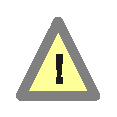
\includegraphics[width=0.6\textwidth]{../../_common/fig/symbols_warning.eps}   
\end{minipage}
\begin{minipage}{0.8\textwidth}
The C++ library \verb!libcpplib.a! is platform-specific, \ie{} you cannot re-use the file when switching between operating systems and/or compiler versions. Disregard of this may yield an executable with subtile bugs which are very hard to trace. Thus, the library must always be re-build after a new installation of the \software{echse} software and each time the C++ compiler is upgraded. The re-build should only be skipped if you run a sequence of attempts to build a model engine and compile time really matters.
\end{minipage} \\

The build scripts provide some basic error checking. If yout get rather lengthy error messages, possible several pages, this indicates a compiler problem. Please make sure that (1) you have the complete source code for the model engine you try to build, (2) the code generator ran without reporting errors, (3) the C++ library was re-build, and (4) the C++ compiler is properly installed.



%%%%%%%%%%%%%%%%%%%%%%%%%%%%%%%%%%%%%%%%%%%%%%%%%%%%%%%%%%
%%%%%%%%%%%%%%%%%%%%% LISTS %%%%%%%%%%%%%%%%%%%%%%%%%%%%%%
%%%%%%%%%%%%%%%%%%%%%%%%%%%%%%%%%%%%%%%%%%%%%%%%%%%%%%%%%%
\clearpage
\fancyhead[LE,RO]{\bfseries\thepage}
\fancyhead[RE]{\bfseries List of figures}
\fancyhead[LO]{\bfseries List of figures}
\addcontentsline{toc}{chapter}{List of figures}
\listoffigures

\clearpage
\fancyhead[LE,RO]{\bfseries\thepage}
\fancyhead[RE]{\bfseries List of tables}
\fancyhead[LO]{\bfseries List of tables}
\addcontentsline{toc}{chapter}{List of tables}
\listoftables

%%%%%%%%%%%%%%%%%%%%%%%%%%%%%%%%%%%%%%%%%%%%%%%%%%%%%%%%%%
%%%%%%%%%%%%%%%%%%%%% BIBLIOGRAPHY %%%%%%%%%%%%%%%%%%%%%%%
%%%%%%%%%%%%%%%%%%%%%%%%%%%%%%%%%%%%%%%%%%%%%%%%%%%%%%%%%%

\clearpage

\twocolumn

\fancyhead[LE,RO]{\bfseries\thepage}
\fancyhead[RE]{\bfseries Bibliography}
\fancyhead[LO]{}
\addcontentsline{toc}{chapter}{Bibliography}
\bibliographystyle{../../_common/elsarticle-harv}
\bibliography{/home/dkneis/literature/jabref/bib_hydrologicalModeling,/home/dkneis/literature/jabref/bib_diplomaAndDiss}

%%%%%%%%%%%%%%%%%%%%%%%%%%%%%%%%%%%%%%%%%%%%%%%%%%%%%%%%%%
%%%%%%%%%%%%%%%%%%%%% THE APPENDIX %%%%%%%%%%%%%%%%%%%%%%%
%%%%%%%%%%%%%%%%%%%%%%%%%%%%%%%%%%%%%%%%%%%%%%%%%%%%%%%%%%

\onecolumn

\chaptermark{A}
\clearpage
\fancyhead[LE,RO]{\bfseries\thepage}
\fancyhead[RE]{\bfseries Appendix}
\fancyhead[LO]{}
\addcontentsline{toc}{chapter}{Appendix}
\appendix

\chapter{Setting environment variables} \label{chap:appendix:envVars}
\renewcommand{\tabdir}{appendix/envVars/envVars/tab}
\renewcommand{\figdir}{appendix/envVars/envVars/fig}

%%%%%%%%%%%%%%%%%%%%%%%%%%%%%%%%%%%%%%%%%%%%%%%%%%%%%%%%%%%%%%%%%%%%%%%%%%%%%%%%
\section{Linux} \label{sec:appendix:envVars:linux}

\begin{enumerate}
  \item Open the shell initialization file in your home directory. On an Ubuntu system, this is \par \hspace{5mm} \verb!/home/user_name/.bashrc! \par Note that files whose names start with a dot are typically hidden.
  \item To set a new variable, add a line like \par \hspace{5mm} \verb!export myVar=value! \par to the file. Don't use spaces before/after the '=' character.
  \item Save the file.
\end{enumerate}

To check your edits, open a \textbf{NEW} shell and try the following:
\begin{itemize}
  \item Enter \verb!echo $myVar! to display variable \verb!myVar!.
  \item Alternatively, enter the \verb!env! command to display all active variables.
\end{itemize}

In some situation it may be useful to update the \verb!PATH! environment variable. The contents of this variable determines where the operation system searches for executable files. In order to add a path name to the \verb!PATH! variable, append a line like \verb!export PATH=$PATH:xxx! to the shell initialization file (see above). The colon is used to separate the added value (\verb!xxx! in this example) from the existing ones.

Note that the value assigned to the \verb!PATH! variable may contain references to other environment variables.

%%%%%%%%%%%%%%%%%%%%%%%%%%%%%%%%%%%%%%%%%%%%%%%%%%%%%%%%%%%%%%%%%%%%%%%%%%%%%%%%
\section{Windows} \label{sec:appendix:envVars:windows}

The following instructions should be applicable to most modern versions of Windows. The exact location of the dialog that allows for the manipulation of environment variables may vary, however.

\begin{enumerate}
  \item
  \begin{itemize}
    \item Windows XP: Click 'Start' $\rightarrow$ 'Control Panel', $\rightarrow$ 'Performance and Maintenance' $\rightarrow$ 'System'.
    \item Windows 7: Click 'Start' $\rightarrow$ 'Control Panel', $\rightarrow$ 'System and Security' $\rightarrow$ 'System' $\rightarrow$ 'Advanced system settings'.
  \end{itemize}
  \item Go to the 'Advanced' tab and click 'Environment Variables'.
  \item Locate the section with 'User variables'. These are the variables you can set/edit without administrator priviliges.
  \item Click 'New' to add a new variable (or 'Edit' or 'Delete' to modify/delete existing ones).
\end{enumerate}

To check your edits, open a \textbf{NEW} shell and try the following:
\begin{itemize}
  \item Enter \lstinline!echo \%myVar\%! to display variable 'myVar'.
  \item Alternatively, enter the \lstinline!set! command to display all active variables.
\end{itemize}

It is sometimes necessary to update the \verb!PATH! environment variable. The contents of this variable determines where Windows searches for executable files. An update is usually required when installing software which does not use the Windows registry. In such cases, you typically need to add the name of the directory where the newly installed executable(s) reside to the existing value of the \verb!PATH! variable. You best append the directory name at the very end of the using a semicolon as separator. 

Consider the following example: If the \verb!PATH! variable already contains the string \verb!c:\program files\soft1! and you installed a software \verb!xy! with the executable(s) in \verb!f:\myPrograms!, the contents of your updated \verb!PATH! variable should be \verb!c:\program files\soft1; f:\myPrograms!.

Note that the value assigned to the \verb!PATH! variable may contain references to other environment variables. This is restricted to variabes of the same category, however, \ie{} you cannot mix system-variables and user-variables.


%%%%%%%%%%%%%%%%%%%%%%%%%%%%%%%%%%%%%%%%%%%%%%%%%%%%%%%%%%
%%%%%%%%%%%%%%%%%%%%% THE INDEX %%%%%%%%%%%%%%%%%%%%%%%%%%
%%%%%%%%%%%%%%%%%%%%%%%%%%%%%%%%%%%%%%%%%%%%%%%%%%%%%%%%%%

\twocolumn

\clearpage
\fancyhead[LE,RO]{\bfseries\thepage}
\fancyhead[RE]{\bfseries Index}
\fancyhead[LO]{}
\addcontentsline{toc}{chapter}{Index}
\printindex

\end{document}
